\newpage
\section{Использование системных вызовов из пользовательского кода}

Для отслеживания обращений к системным вызовам используется код из листинга 1. Результаты его работы представлены на рисунке 2.

\lstinputlisting[language=C++, caption={демонстрация использования системных вызовов (src/syscalls/sched.c)}]
{../../src/syscalls/sched.c}

\begin{figure}[h!]
\centering
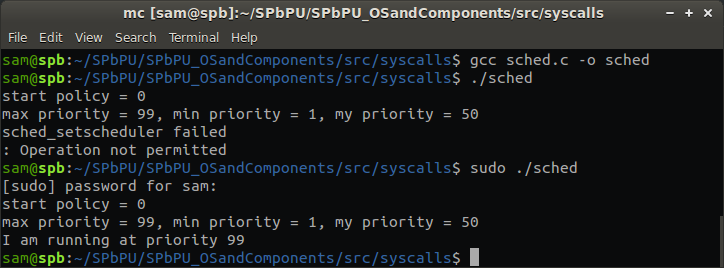
\includegraphics[scale=0.7]{res/pic002}
\caption{Результат запуска программы sched}
\end{figure}

Для отслеживания системных вызовов будем использовать strace. Эта утилита отслеживает системные вызовы и представляют собой механизм трансляции, обеспечивающий интерфейс между процессом и операционной системой (ядром). Эти вызовы могут быть перехвачены и прочитаны, что позволяет лучше понять, что процесс пытается сделать в заданное время. Перехватывая эти вызовы, можно добиться лучшего понимания поведения процессов, особенно в процессе отладки. Функциональность операционной системы, позволяющая отслеживать системные вызовы, называется ptrace. Strace вызывает ptrace и читает данные о поведении процесса, возвращая отчет.

Отчёт по работе программы sched представлен в листинге 2.

\lstinputlisting[language={},caption={Протокол системных вызовов}]{res/strace.rep}

Как можно видеть в листинге 2, помимо изучаемых программа делает ещё множество стронних вызовов (к примеру, подгружает системные библиотеки). Но в последних строчках просисходят ожидаемые системные вызовы.